\chapter{准备知识}

\section{数据立方}
数据立方(Data Cube)的实现是联机分析处理(OLAP)中一项非常关键并受到业界广泛关注的技术。为有效支持 OLAP应用,Jim Gray 等人于 1996 年提出一种多维数据存储模型 —— 数据立方 \cite{gray1997data}。该结构存储了事实表中各维属性间的所有组合对应的聚集计算结果,即各个维度组合的 GROUP BY 结果。在 OLAP 术语中,聚合属性称为维属性, 被合计的属性称为度量属性。

根据数据立方计算和存储所采用的不同表达形式,可以将不同的数据立方实现算法分成以下 4 种技术类别
\begin{enumerate}
\item 采用传统关系型视图的 ROLAP 技术 \cite{morfonios2007rolap}
\item 采用多维数组的MOLAP技术 \cite{zhao1997array}
\item 采用类树型数据结构的基于图(Graph-Base)技术 \cite{zhao2011graph}
\item 采用多种内存表达方式的近似计算技术 \cite{kamatdistributed}
\end{enumerate}

但鉴于以下3点原因,本文研究在 ROLAP 技术下的数据立方实现技术。
\begin{enumerate}
\item 现在业界内大部分的数据立方研究技术都是基于 ROLAP 开展的
\item MOLAP 以及 Graph-Base,基于 ROLAP 的数据立方实现算法能够容易的与目前存在的大多数关系引擎结合,使得他们能够以更低的代价转化为强而有力的 OLAP 工具
\item 相对于近似计算,基于 ROLAP 的方法能够生成并存储更精细的结果集合,使得它们在运行期间更容易管理
\end{enumerate}

如图\ref{fact_table_data_cube} 所示,(a) 为事实表 R, A、B、C 为它的维属性,M 为它的度量z属性。(b) 展示的是基于事实表 R 构建的数据立方。(b)中的每个视图代表的就是某个特定维属性组合的 GROUP BY 结果。所有 GROUP BY 结果的组合即构成数据立方。

\begin{figure}[!htb]
\centering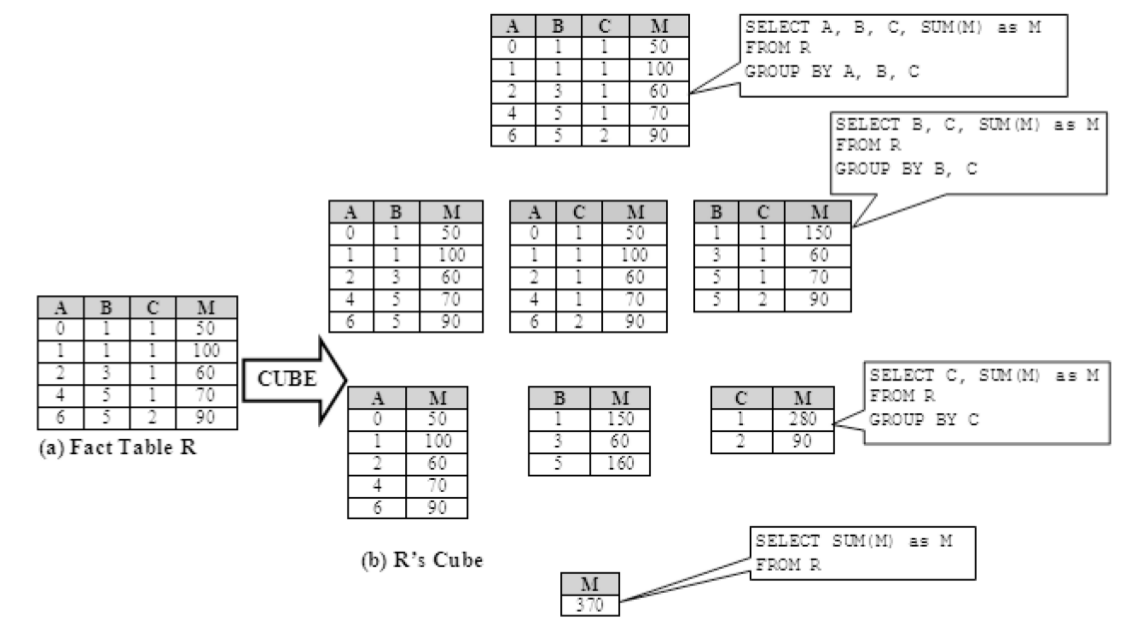
\includegraphics[width=6in]{picture/ch_preliminary/fact_table_data_cube} 
\caption{事实表与数据立方}\label{fact_table_data_cube} 
\end{figure} 

\section{Lattice, Region, Group}

对于图\ref{fact_table_data_cube} 中的所有GROUP BY,可用另一种方式表示,如图\ref{abc_lattice} 所示,这种结构称为 Lattice。

\begin{figure}[!htb]
\centering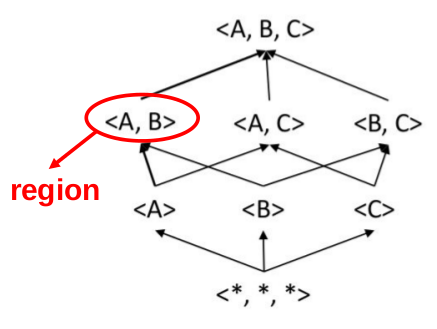
\includegraphics[width=2in]{picture/ch_preliminary/abc_lattice} 
\caption{ABC Lattice}\label{abc_lattice} 
\end{figure} 

在这个lattice中,有维属性对应的所有 GROUP BY 类型,每个节点表示一种 GROUP BY 类型,箭头连接的两个节点表示它们有父子关系。在lattice中的每个节点称为一个数据小方 (Cuboid),数据小方也可被称为一个Region,也就是一种 GROUP BY 类型。在之后的章节中,数据小方与 region 这两种称呼均会被提及。

一个 region 内有多个 group。group 指的是一个
Region中带有具体值的 Group By。例如图\ref{fact_table_data_cube} 中的 GroupBy(A),就有表\ref{groupby_a_table}的结果。

\begin{table}[hbtp]
\begin{center}
\begin{tabular}{|c|c|}
\hline 
A & M \\ 
\hline 
0 & 50 \\ 
\hline 
1 & 100 \\ 
\hline 
2 & 60 \\ 
\hline 
4 & 70 \\ 
\hline 
6 & 90 \\ 
\hline 
\end{tabular} 
\end{center}
\caption{GroupBy(A)}\label{groupby_a_table}
\end{table}

在表\ref{groupby_a_table}中,Region \textless A\textgreater 中有5个Group,分别是Group(A=0), Group(A=1), Group(A=2), Group(A=4), Group(A=6)。

从lattice中可见,当一个事实表有 D 个维属性时,它对应的数据立方就会有${2}^{D}$个region,也即有 ${2}^{D}$ 种不同类型的 GROUP BY 的查询。最简单直接(Naive)的数据立方实现方法,会对每个region进行独立计算并把结果存储起来。对于一张事实表,随着他的维属性数量的增加,它相对应的数据立方的计算与存储代价就会呈指数增长。于是,在 ROLAP 中,如何从立方计算、立方存储这两个角度高效地实现数据立方已成为业界内广泛讨论的一个研究课题。


\section{度量}

度量,即对GROUP BY的多条数据进行计算,例如SUM,AVEG,MEDIAN等。

度量函数一般分为三大类, 分别是分布式度量(Distributive),线性度量(Algebraic)和整体性度量(Holistic)。

以下使用一个二维的数据集$\left\{ {X}_{ij}|i=1,...I; j=1,...J \right\}$分别说明这三种度量函数的区别。

\begin{itemize}

\item \textbf{分布式度量}

对于分布式度量函数 F(),如果存在一个辅助函数 G() 能令 $F(\text\{ {X}_{i,j} \text\}) = G(\text\{ F(\text\{ {X}_{i,j}|i=1,...,I \text\})|j=1,...J \text\})$,则度量函数 F() 为分布式度量函数。常见的分布式度量函数有 COUNT(), MIN(), MAX(), SUM()。大部分分布式度量函数中 $F=G$,但COUNT() 除外。在COUNT()度量函数中,$G=SUM()$。

\item \textbf{线性度量}

对于线性度量函数 F(),如果存在辅助两个函数 G() 和 H(),其中 G() 的输出结果是确定数量固定的 M 条记录,并且满足$F(\text\{ {X}_{i,j} \text\}) = H(\text\{ G(\text\{ {X}_{i,j}|i=1,...,I \text\})|j=1,...J \text\})$。常见的线性度量函数有Average(),MaxN(),MinN(),standard deviation等。例如对于Average(),函数G()的输出是子集的和以及数量,H()函数则把将各个子集的和相加再除以数量的总和。线性度量的关键是,函数G()的输出结果的数据多少是确定的。例如Average(),无论数据怎么划分,函数G()的输出都是两个数,一个是和,另一个是数量。

\item \textbf{整体性度量}

对于整体性性度量函数 F(),其中间结果,即各个子集的计算结果的数据量大小是不确定的。常见的整体性度量有Median(), Mode(), RANK(), DISTINCT()等。

\end{itemize}

之所以要对度量函数进行分类是因为其会影响数据的划分。论文研究的是分布式环境下数据立方的计算,因此数据划分是必然的。对于以上三种度量,在分布式度量与线性度量下,数据无论如何划分,使用辅助函数都能计算出最终结果,并且中间结果的数据大小是确定的。但对于整体性度量,虽然数据不能随意划分,或者数据的随意划分对其计算的意义并不大,但并不代表数据不能划分。在后面的章节中会提到,对于整体性度量按照一定的方法对数据进行划分,也能令中间结果的数据大小是确定的。

\section{MapReduce}

MapReduce是Google提出的一个软件架构,用于大规模数据集的并行运算。MapReduce的数据流动如图 \ref{mr_data_flow} 所示。它的整个执行流程分为以下几个步骤:

\begin{enumerate}
\item 输入的数据被划分成块分派到各个Map任务中。
\item Map对输入的数据块处理后,排序并写到磁盘上,输出格式为键值对(Key-Vavlue)。
\item 在Merge阶段从各个Map获取具有相同Key值的数据。
\item 在Sort阶段,将上一阶段合并的结果排序后发到对应的Reducer上。
\item Reducer对输入的键值对进行处理后输出。具有相同Key值的数据会被分派到同一个Reducer任务上。
\end{enumerate}

\begin{figure}[!htb]
\centering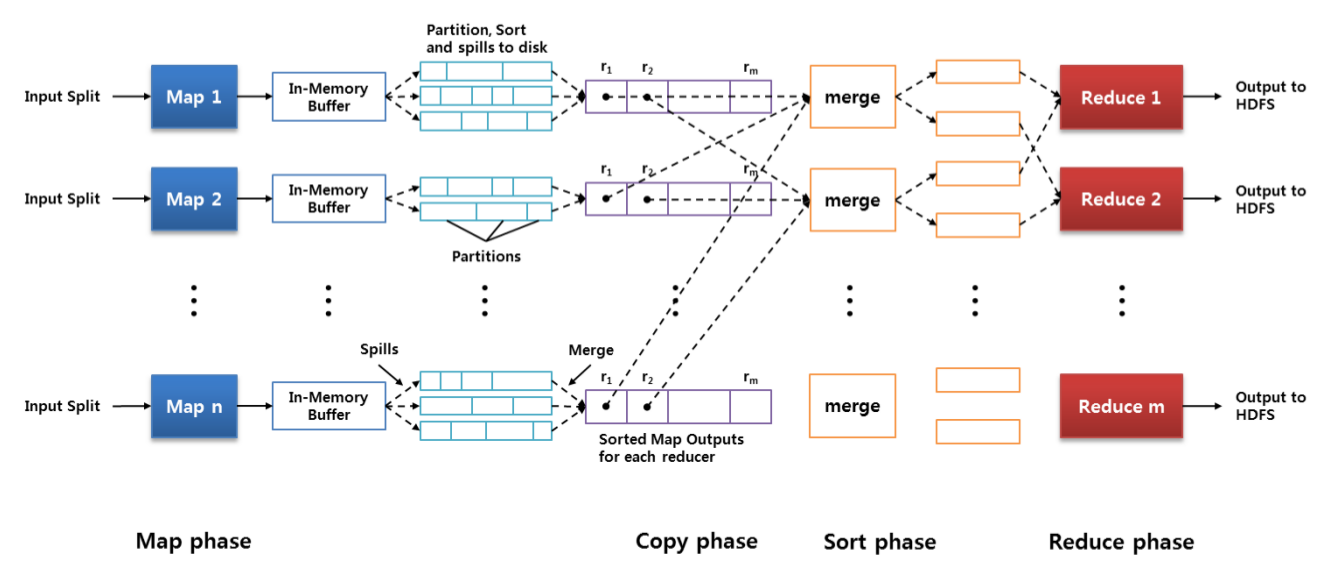
\includegraphics[width=6in]{picture/ch_preliminary/mr_data_flow} 
\caption{MapReduce的数据流动}\label{mr_data_flow} 
\end{figure} 

图\ref{mr_word_count}是用MapReduce进行单词统计的例子。

\begin{figure}[H]
\centering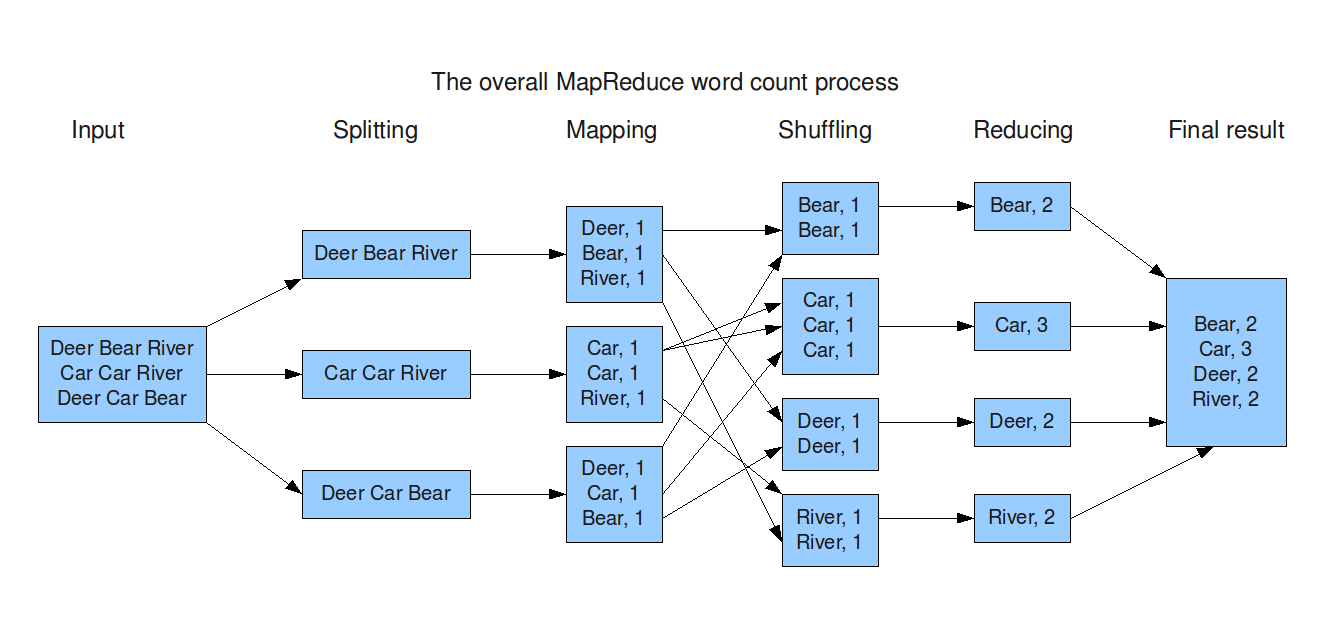
\includegraphics[width=6in]{picture/ch_preliminary/mr_word_count} 
\caption{MapReduce单词统计例子}\label{mr_word_count} 
\end{figure} 



